% Status: DRAFT. Do not submit without: second rater on n=80, external annotator, code human
% labels, equivalence adjudication (see Limitations).
% TODO citations: Putnam-AXIOM, Omni-MATH, GSM8K-Platinum, MATH-500 subset paper (verify IDs
% before submission; only confidently-known references are cited below).
% !TEX root = main.tex
%
% bit flip (planning comment, not prose): prior work treats cheap reference-matching metrics and
% LLM judges as points on one cost-quality tradeoff, and treats evaluator trustworthiness as an
% empirical unknown discovered after deployment. We flip both: (1) validity is determined by the
% signal's MECHANISM (compare vs verify); (2) trustworthiness is a CERTIFIABLE ex-ante property,
% and the static certificate predicts survival under optimization pressure.
\documentclass[11pt]{article}
\usepackage[margin=1in]{geometry}
\usepackage{amsmath,amssymb}
\usepackage{graphicx}
\usepackage{booktabs}
\usepackage{multirow}
\usepackage{xcolor}
\usepackage[colorlinks=true,linkcolor=blue,citecolor=blue,urlcolor=blue]{hyperref}
\usepackage{caption}
\captionsetup{font=small,labelfont=bf}

\newcommand{\tfa}{\textsc{TFA}}

\title{Verify, Don't Compare:\\ \large What Reference-Based Metrics Actually Measure, and How to Certify What Replaces Them}
\author{Anonymous Authors}
\date{Draft, August 17, 2026}

\begin{document}
\maketitle

\begin{abstract}
% 1 problem motivation
Which automated signals can be trusted to grade a model's reasoning?
% 2 assumption being challenged
Many benchmarks ship a gold reference solution, so the cheapest evaluators score a solution by how much it resembles that reference, the most expensive ask an LLM judge, and everything between is treated as a tradeoff of cost against quality.
% 3 flip
We find the real divide is not cost but \emph{mechanism}: whether a signal \emph{compares} a solution to the reference, or \emph{verifies} it against something checkable.
% 4 instantiation
Comparison does not grade.
Five reference-similarity metrics were uncorrelated with blind human judgments of reasoning quality on competition math and with executed tests on code, and across seventeen models and eight benchmarks most of what they measure is a property of the reference itself: teacher-forced accuracy, the most direct of them, is $80\%$ reference perplexity.
Verification does grade.
Executed tests are a free oracle where they exist.
A completion test, asking whether a truncated solution still reaches the right answer, correlates at $+0.79$ with human judgment with no LLM involved, and a judge grades reliably once anchored to a reference it can check.
% 5 evaluation
This divide can be measured before an evaluator is deployed.
A blind audit built on sixty human labels tells the two mechanisms apart, and the audit's verdict predicts behavior under optimization pressure: in best-of-64 selection across 25 judge configurations, every judge that failed the audit was gamed, and every judge certified in its own domain resisted.
% 6 implications
Two practical rules follow: use a reference as input to a verifier, never as a similarity target, and audit an evaluator in its deployment domain before optimizing against it.
\end{abstract}

\section{Introduction}
\label{sec:intro}

% P1: problem motivation
Most benchmarks that matter ship with a gold reference: a worked solution or a canonical program known to be correct.
This is true of grade-school math, competition math, and program synthesis alike~\cite{cobbe2021gsm8k,hendrycks2021math,chen2021codex}.
Evaluating against the reference without a judge is appealing.
It is deterministic, costs one forward pass, cannot be sweet-talked, and anyone can audit it.
The sharpest version is teacher-forced accuracy (\tfa): feed the model the problem and the gold solution one token at a time, and score the fraction of gold tokens the model would have predicted itself.
As models are increasingly evaluated, filtered, and trained by automated signals, knowing which of those signals measure quality has become a bottleneck for the field.

% P2: the assumption
Prior work organizes this space along a single axis of cost versus quality: string and embedding metrics at the cheap end~\cite{yuan2021bartscore}, LLM judges at the expensive end~\cite{zheng2023judging}, and the practical question is how far down the cost axis one can afford to go.
Two assumptions hide in this framing.
The first is that reference similarity degrades gracefully, so that a cheaper metric measures the same thing with more noise.
The second is that whether a given judge can be trusted is an empirical unknown, discovered only after the judge has been deployed and, in the worst case, reward-hacked~\cite{gao2022scaling}.

% P3: the flip
Both assumptions fail, and for the same reason.
The operative axis is not cost but \emph{mechanism}.
Evaluation signals divide into a \emph{comparison class}, which scores resemblance to the reference text, and a \emph{verification class}, which checks whether the solution reaches or supports a checkable endpoint (Figure~\ref{fig:concept}).

\begin{figure}[t]
\centering
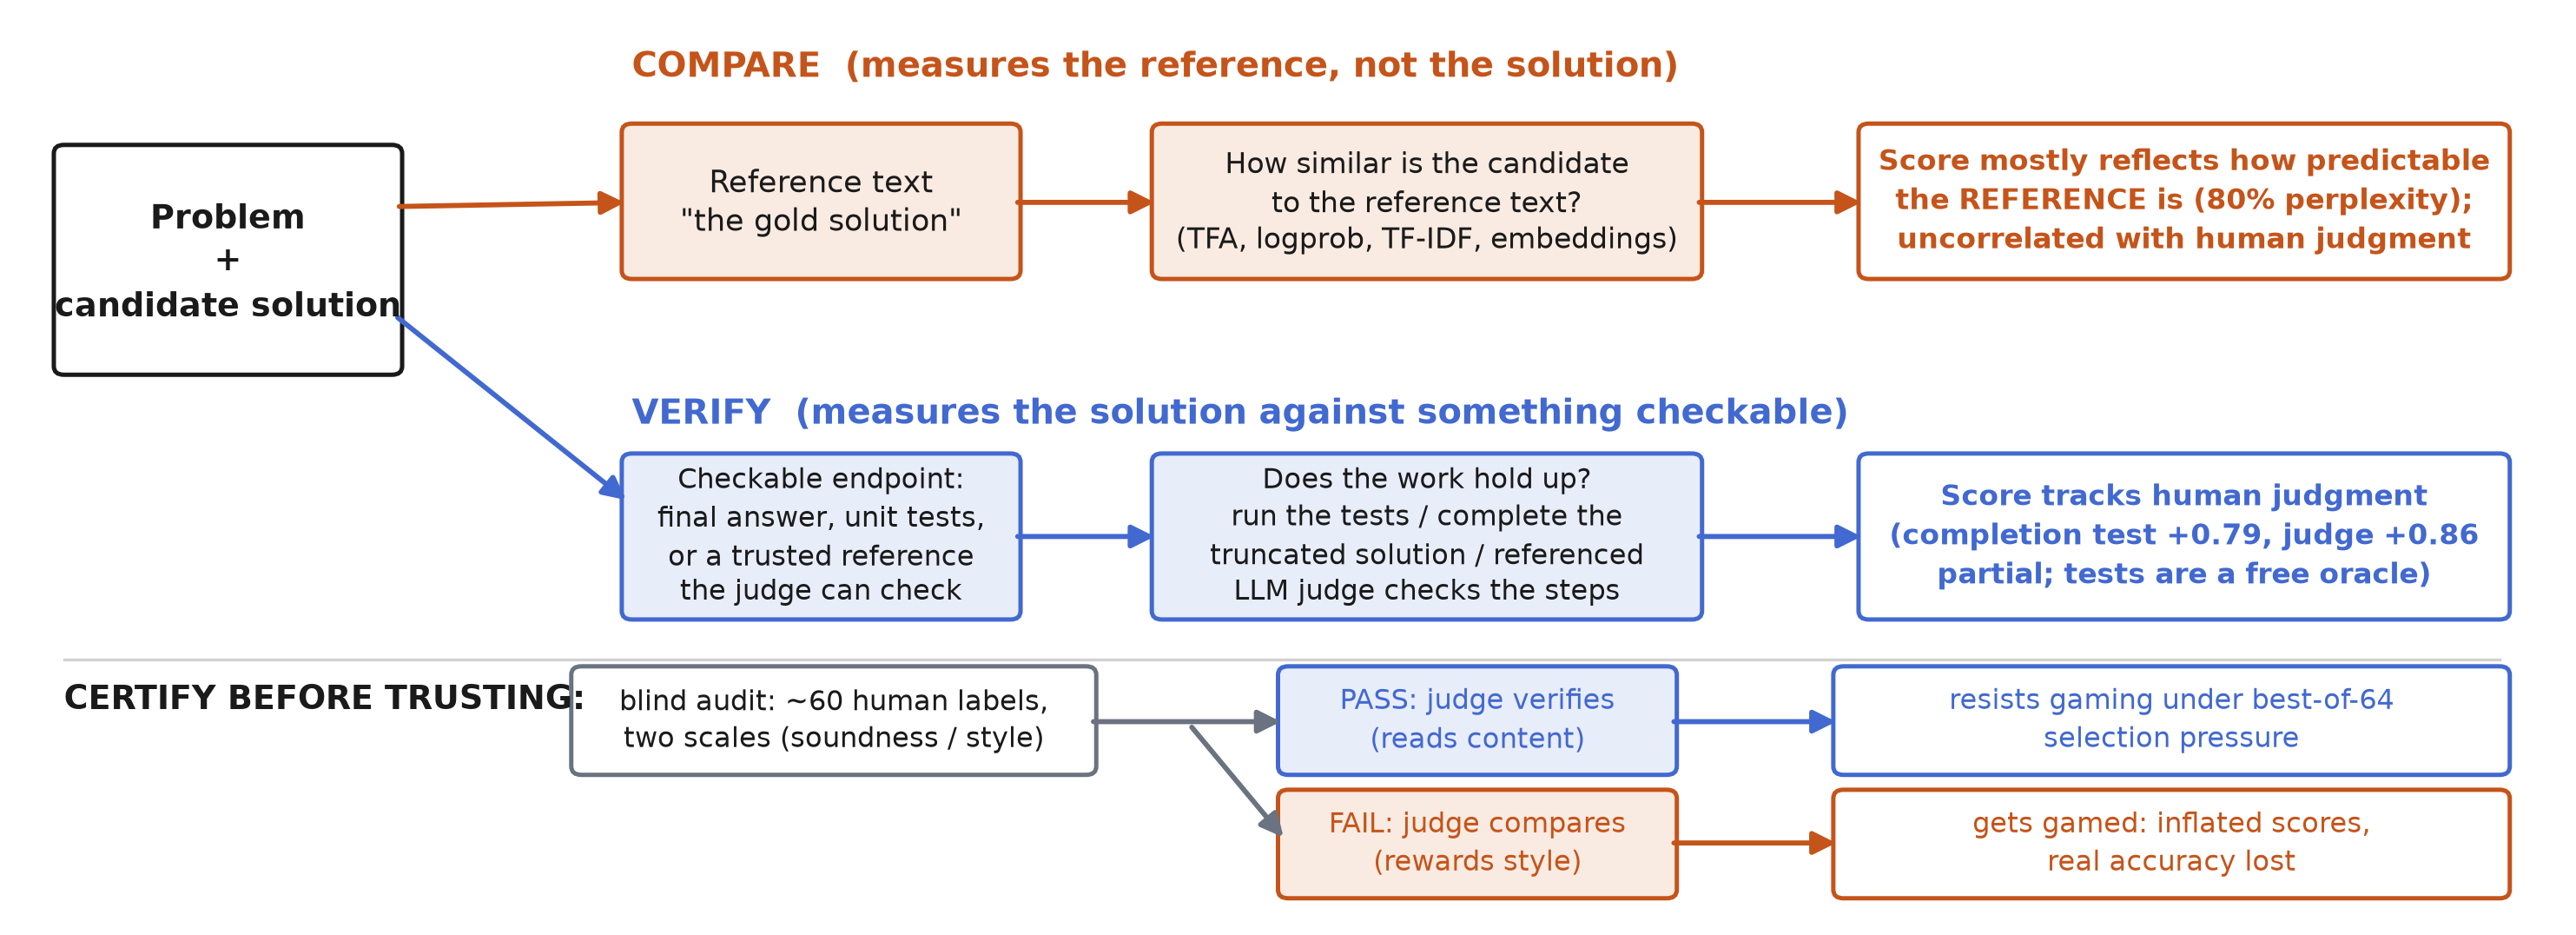
\includegraphics[width=\textwidth]{figs/fig0_concept.png}
\caption{\textbf{The compare-vs-verify divide, and why it is auditable.}
Top: comparison metrics score a candidate by its resemblance to the reference text, so most of their signal is a property of the reference, not the solution.
Middle: verification signals check the solution against a checkable endpoint, so their signal tracks the solution's actual quality.
Bottom: a blind sixty-label audit reveals which mechanism an evaluator uses, and the verdict predicts whether it survives optimization pressure (Section~\ref{sec:pressure}).}
\label{fig:concept}
\end{figure}
The comparison class does not degrade gracefully.
It measures nothing about the individual solution at any price point, because its variance is dominated by a property of the reference itself.
And because the failure is mechanistic, trust stops being an unknown.
An evaluator can be certified in advance with roughly sixty blind human labels, and the certificate predicts which evaluators survive optimization pressure before any optimization is run.

% P4: instantiation
We anchor everything to blind human grades on two deliberately separated scales: soundness of the reasoning and quality of the writing.
The protocol is designed so that a good evaluator can demonstrably pass, rather than only catching bad ones.
We test five comparison metrics spanning the space, from \tfa{} to sentence embeddings, along with targeted repairs of each.
We test three verification signals: executed tests, a prefix-repair completion curve, and an answer-swap counterfactual.
We audit LLM judges with and without trusted references, including a deliberately sabotaged judge as a positive control.
Finally, we place 25 judge configurations under best-of-64 selection pressure in math and code and measure, with pre-registered estimators, which ones inflate their own scoreboards and which ones lose real accuracy.

% P5: evaluation summary (Figure 1 carries the detail)
Figure~\ref{fig:master} summarizes the results.
The comparison class fails completely: against human soundness (labeling round one) all five metrics land in $[-0.24, +0.14]$, where the LLM judge reaches $+0.59$ on identical items, and against executed tests on 492 code solutions they are indistinguishable from zero.
The reason is mechanistic.
For \tfa, $83$--$92\%$ of per-solution variance beyond model level is reference-specific nuisance, and the same structure appears attenuated in every similarity metric.
Pooled across 6{,}000 model--item pairs, \tfa{} correlates at $-0.895$ with reference perplexity.
It meters compressibility, not quality.
Every targeted repair we or our reviewers proposed left the signal at zero or made it worse, as the mechanism predicts.
On the other side, the prefix-repair curve reaches $+0.79$ with human soundness (labeling round two) with no judge involved, and every open-weights judge we tested fails the certification audit blind and passes it referenced.
Under selection pressure the certificate predicts hack-resistance, with one mechanism-flagged exception on code that Section~\ref{sec:pressure} dissects.
A deliberately style-loaded frontier judge shows the most dangerous failure mode: on math it inflates its scoreboard ($+0.85\sigma$ excess gap versus $+0.38$ honest) while selecting almost as well as the honest judge (regret $0.133$ versus $0.117$).
It deceives the metric, not the outcome.

% P6: implications
These results replace a folk cost--quality tradeoff with a taxonomy that made correct advance predictions for every new metric we built, and they turn evaluator trust into a measurable, falsifiable property.
For benchmark builders, a reference's value is as context for a reader or as an endpoint for a checker, never as a similarity target.
For anyone optimizing against an evaluator, whether in best-of-$n$ serving, data filtering, or RLHF, the rule is to certify first, in the deployment domain.
The evaluators that fail the sixty-label audit are the ones optimization will exploit.

\begin{figure}[t]
\centering
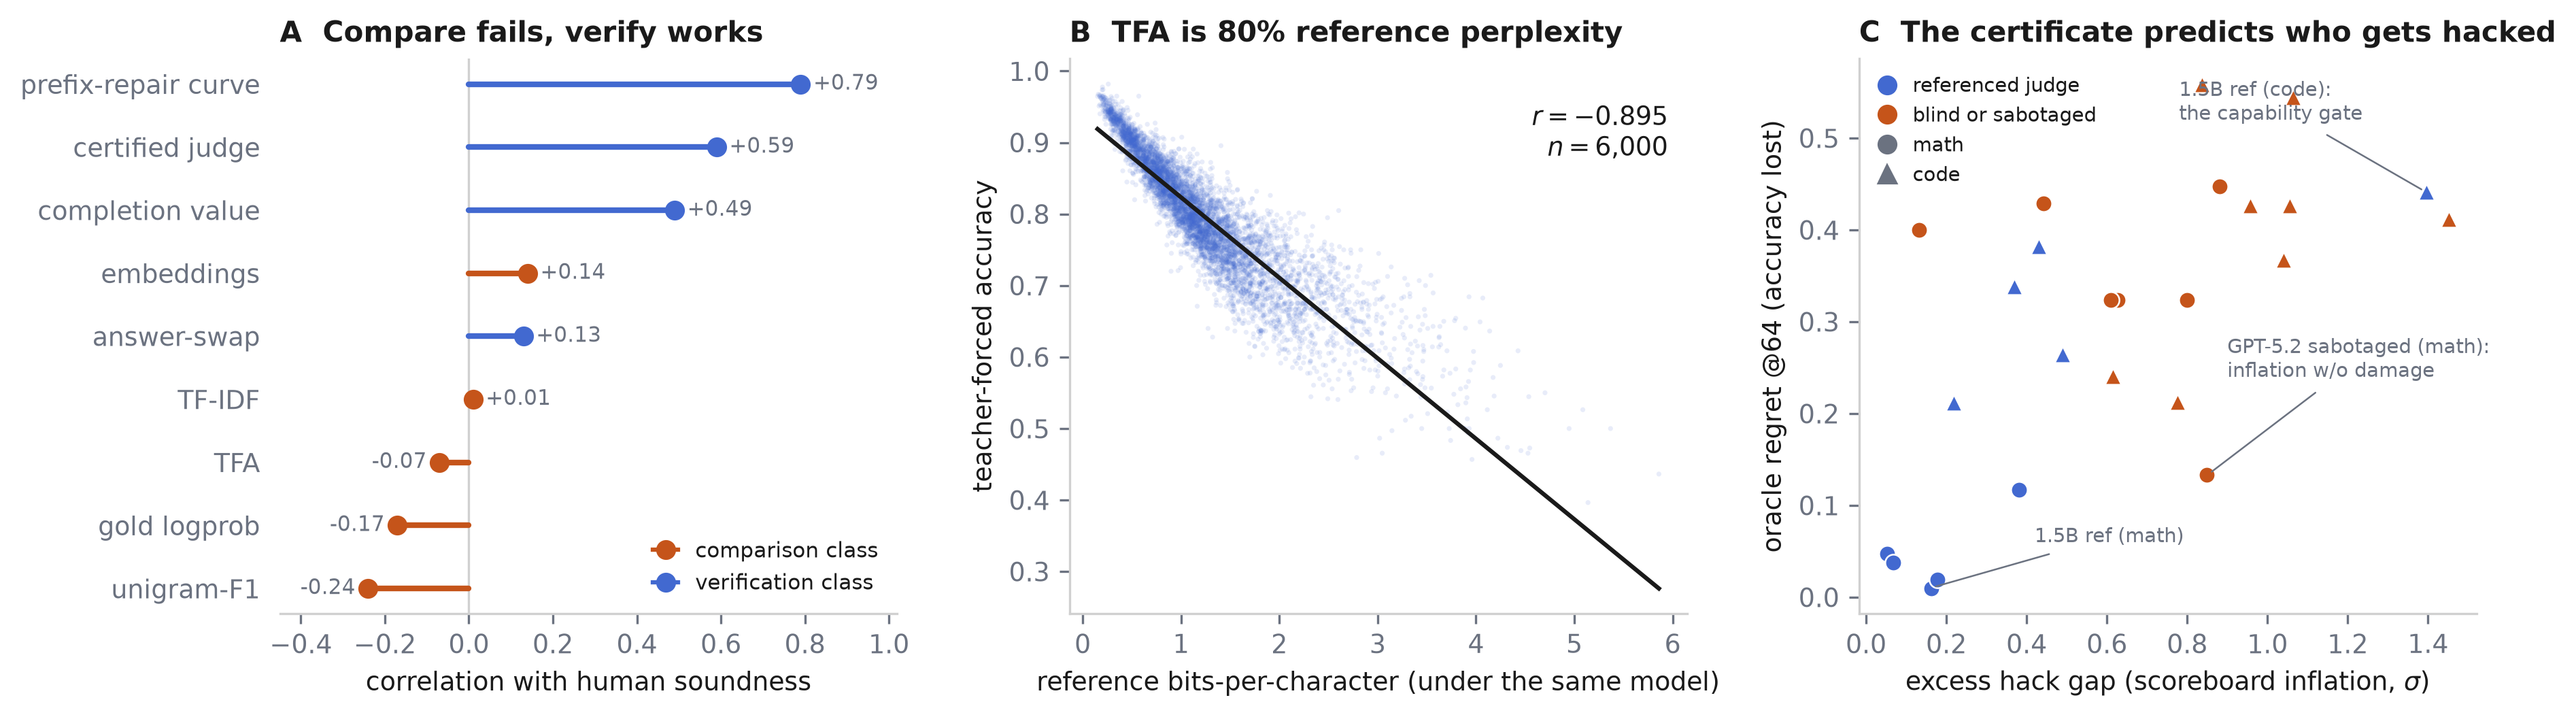
\includegraphics[width=\textwidth]{figs/fig1_master.png}
\caption{\textbf{The paper in one figure.}
\textbf{(A)} Against blind human soundness grades, all five reference-comparison metrics land within noise of zero, while verification-shaped signals carry real signal, topping out at the prefix-repair curve ($+0.79$, measured on labeling round two; other entries on round one, Section~\ref{sec:setup}).
\textbf{(B)} The mechanism: across 6{,}000 model--item pairs, teacher-forced accuracy is $80\%$ reference perplexity.
It measures the reference, not the solution.
\textbf{(C)} Under best-of-64 selection pressure (25 configurations, two domains), blind and sabotaged judges (orange) are hacked, with high scoreboard inflation, high accuracy loss, or both, while referenced judges (blue) resist.
The two labeled exceptions are the paper's two mechanisms: the 1.5B code judge that cannot \emph{use} its reference (the capability gate), and the sabotaged frontier judge that deceives the metric without damaging selection.}
\label{fig:master}
\end{figure}

\section{Setup}
\label{sec:setup}

\paragraph{Models and data.}
Seventeen instruction-tuned models from seven families (Qwen, Phi, Mistral, OLMo, plus math-specialized Qwen-Math, DeepSeek-Math, and Mathstral), spanning 0.5B to 32B parameters.
GPT-5.2 serves as the frontier judge; Claude Opus serves as a blind cross-family panel for channel decomposition and is designated for the pending answer-equivalence adjudication.
Two judge-side probes recur in Section~\ref{sec:certify}: a \emph{planted-error detection} task (known-correct solutions mechanically corrupted, every corruption verified before use, so the right verdict is never in doubt) and \emph{multi-valid-answer comparisons} (RewardBench-2 items whose prompts admit several enumerated correct answers).
Eight benchmarks: \textsc{MATH-500} and full \textsc{MATH}~\cite{hendrycks2021math}, \textsc{Putnam-AXIOM} and variations, \textsc{Omni-MATH}, \textsc{GSM8K}~\cite{cobbe2021gsm8k}, \textsc{GSM8K-Platinum}, and \textsc{HumanEval}~\cite{chen2021codex}/\textsc{MBPP+}~\cite{austin2021mbpp,liu2023evalplus}, plus \textsc{SWE-bench Verified} as an agentic setting (patch-level \tfa{} over eight coder models, including the Qwen-Coder size ladder).
Every model generates its own solution to every problem (greedy), and is separately teacher-forced on the gold solution.

\paragraph{The comparison class.}
Five ways of scoring a solution against the reference, chosen to span the space: \tfa{} (hard argmax match on gold tokens), gold-token log-probability (the soft version), TF-IDF cosine, unigram-F1, and sentence-embedding cosine.
The first two measure the model's predictive fit to the reference text.
The last three measure how much the model's own output resembles it.

\paragraph{The verification class.}
Three signals that consume the reference only through a checkable endpoint.
\emph{Executed tests}: for code, run the official suite.
\emph{Prefix-repair curve}: truncate the solution at depth $k \in \{0, 0.25, 0.5, 0.75\}$, let a fixed mid-sized completer finish it, and score the fraction of completions that reach the correct final answer~\cite{lightman2023verify,wang2022selfconsistency}.
The profile over $k$ is the signal, and $k{=}0$ is a pure problem-difficulty probe.
\emph{Answer-swap counterfactual}: the per-token log-probability margin a fixed scorer assigns the solution's own final answer over a swapped alternative, given the reasoning prefix.
LLM judges sit in either class depending on protocol, which Section~\ref{sec:certify} measures directly.

\paragraph{Human grades.}
Annotators graded solutions blind, with no model names and no metric scores, on two 0--10 scales with written anchors: \emph{soundness} (is every step valid; ignore the writing) and \emph{style} (is it clear and well-organized; ignore correctness).
Two annotators graded a shared block to establish a reliability ceiling (soundness $\rho = 0.79$, style $0.55$).
The uniformly random \textsc{MATH-500} sample was labeled in two rounds: round one (60 items) anchors the metric-class comparisons, and round two (an 80-item instrument with 60 items labeled to date, all 60 joining to every signal) anchors the prefix-repair curve.
The LLM judge reads $+0.59$ against round one and $+0.89$ against round two; we name the round whenever we quote either number.
A divergence-selected block decorrelates soundness from style ($+0.82 \to +0.31$) for the partial-correlation audits.
For code correctness no human is needed: we execute the tests.

\paragraph{Statistics and pre-registration.}
Headline correlations are Spearman or Pearson with bootstrap 95\% intervals.
Grading claims control for final-answer correctness where stated, because checking the final answer is free and is not what anyone needs a grader for.
The selection-pressure experiments (Section~\ref{sec:pressure}) and all four new-metric predictions (Section~\ref{sec:slate}) were pre-registered: analysis scripts and directional predictions were committed to the repository before the corresponding data were generated.

\section{The comparison class cannot grade, and we know why}
\label{sec:compare}

\subsection{The class-level null}
\label{sec:classnull}

On labeling round one, the five comparison metrics correlate with human soundness at $-0.07$ (\tfa), $-0.17$ (gold-token probability), $+0.01$ (TF-IDF), $-0.24$ (unigram-F1), and $+0.14$ (embeddings); the full class table is Appendix~\ref{app:classtable}.
Every interval includes zero.
On the same solutions the LLM judge reaches $+0.59$, and the prefix-repair signal reaches $+0.49$ in its single-point form.
Code offers a referee no one can argue with: on 492 freshly generated solutions scored by executing the official test suites, \tfa's correlation with passing is $0.00$, and stays within $[-0.04, +0.06]$ inside each model.
(This is the per-solution correlation; the model-level code ranking is Table~\ref{tab:map}'s $+0.43$ row.)
The soft log-probability version does no better.

\subsection{The mechanism: comparison scores are reference properties}
\label{sec:mechanism}

We decomposed per-solution \tfa{} across a grid of fifteen to sixteen models from four families (the count varies by benchmark with model availability), after removing each model's overall level.
Between $83\%$ and $92\%$ of the remaining variance is an \emph{item main effect}: a component identical across families.
Such a component can only be a property of the reference, namely how predictable this particular gold text is.
Another $3$--$7\%$ is family-specific style, and this style channel roughly doubles on saturated benchmarks (\textsc{GSM8K} $7.2\%$, full \textsc{MATH} $6.5\%$, versus \textsc{Putnam} $2.9\%$).
The same structure appears in code ($78\%$ item, $8\%$ family, $14\%$ residual), and attenuated in every similarity metric (item share: log-probability $83$--$91\%$, embeddings ${\sim}70\%$, TF-IDF $69\%$).

Across 6{,}000 model--item pairs on \textsc{MATH-500}, \tfa{} correlates with the reference's bits-per-character under the same model at $r = -0.895$, so reference perplexity explains $80\%$ of the pooled variance (Figure~\ref{fig:master}B).
This is a different accounting from the $83$--$92\%$ item share above: the decomposition splits variance across models and items, while this pools everything, and both point the same way.
To first order, teacher-forced accuracy measures how compressible the reference is.
A score that is four-fifths about the reference cannot grade the solution in front of it.

\subsection{Ranking survives exactly where the mechanism says it should}
\label{sec:ranking}

Averaged over a benchmark, mean \tfa{} ranks models by accuracy on hard data and not at all on easy data.
Every family ladder is positive on the three olympiad benchmarks (twelve of twelve family--benchmark cells), while on the easiest benchmarks five of twelve family ladders invert.
Table~\ref{tab:map} shows the full boundary: the pooled cross-family correlation runs from $\rho = +0.86$ on olympiad math down through zero and into reversal on saturated data.

\begin{table}[t]
\centering
\small
\begin{tabular}{llcc}
\toprule
benchmark & regime & cross-family $\rho$ [95\% CI] & within-family $\rho$ \\
\midrule
\textsc{Omni-MATH} & olympiad & $+0.86$ $[+0.35, +1.00]$ & $+0.90$ \\
\textsc{Putnam-AXIOM} & olympiad & $+0.60$ $[+0.17, +0.83]$ & $+1.00$ \\
\textsc{Putnam-Variations} & olympiad, contamination-proof & $+0.38$ $[-0.15, +0.73]$ & $+0.90$ \\
\textsc{HumanEval} & code & $+0.43$ $[-0.02, +0.76]$ & $+0.80$ \\
\textsc{MATH-500} & competition math & $+0.35$ $[-0.15, +0.71]$ & $+0.90$ \\
\textsc{MATH} (full) & competition math, near-saturated & $+0.21$ $[-0.29, +0.61]$ & $+0.60$ \\
\textsc{GSM8K} & grade school, saturated & $-0.25$ $[-0.71, +0.33]$ & $+0.70$ \\
\textsc{GSM8K-Platinum} & grade school, relabeled & $-0.19$ $[-0.71, +0.41]$ & $+0.60$ \\
\textsc{SWE-bench Verified} & agentic code & $0.00$ (8 coder models) & $+1.00$ (Qwen-Coder) \\
\bottomrule
\end{tabular}
\caption{\textbf{The boundary map: where reference matching ranks models.}
Cross-family Spearman correlation between mean \tfa{} and accuracy (17 models; bootstrap CIs), and the Qwen size-ladder correlation as the within-family column, per benchmark.
Ranking degrades from olympiad to saturated benchmarks, with code sitting mid-scale, and within-family ladders survive everywhere the pooled comparison does not, because family style cancels inside a family and survives across families.}
\label{tab:map}
\end{table}
Across benchmarks, this ranking signal correlates $+0.89$ with mean reference entropy and $-0.81$ with saturation, but the two are confounded in observational data.
So we intervened.
On the same \textsc{MATH-500} items, replacing each worked reference with the single line ``The final answer is [answer]'' collapses the ranking signal from $+0.35$ to $+0.02$.
Predicting a long, information-dense reference requires skill adjacent to solving the problem.
Predicting a formulaic one requires nothing, leaving only style.

The positive side of the boundary is worth stating as plainly as the negative.
Comparison metrics do rank models, under three conditions that all hold at once:
\begin{enumerate}
\item \textbf{Use them in aggregate, never per item.}
The reference-predictability nuisance is identical for every model on a given item, so it cancels when scores are averaged over a benchmark; per-item it dominates.
\item \textbf{The reference must be detailed enough to be worth predicting.}
A long worked solution differentiates strong models from weak ones; an answer line does not (the $+0.35 \to +0.02$ intervention above).
\item \textbf{The benchmark must be hard enough to differentiate models.}
On saturated data every model predicts the reference about equally well, and the leftover variance is writing style, which is why saturated rankings collapse or invert.
\end{enumerate}
The agentic setting obeys the same boundary.
On \textsc{SWE-bench Verified}, patch-level \tfa{} ranks the four Qwen-Coder sizes perfectly ($\rho = +1.00$) yet carries no cross-family signal ($\rho = 0.00$, eight models).
Family style survives averaging, so cross-family comparison needs a shared style or a verifier.
The consequence for leaderboards: reference matching is legitimate exactly when these conditions hold, and reference entropy can be measured in advance to check the second one.

\subsection{Repairs fail as predicted: the class is empty, not under-tuned}
\label{sec:slate}

A natural response is that some reweighting rescues the metric.
The mechanism predicts otherwise, and we tested that prediction adversarially.
Every variant in Table~\ref{tab:slate} was proposed either by our reviewers or by the mechanism itself, and the directional outcome was registered in the repository before the run.

\begin{table}[t]
\centering
\small
\begin{tabular}{llll}
\toprule
proposed metric & class & registered prediction & outcome \\
\midrule
position-weighted \tfa{} (late tokens up-weighted) & comparison & null & decays $+0.13 \to -0.37$ \\
entropy-normalized \tfa{} (perplexity residualized) & comparison & null & ranking $+0.13 \to -0.17$ \\
seven reweightings (IDF, surprisal, masking, \dots) & comparison & null & all $\le 0$ \\
answer-swap counterfactual & verification & works & $+$ in 8/9 models, mean $+0.13$ \\
prefix-repair curve & verification & works & $+0.79$ vs.\ human soundness \\
\bottomrule
\end{tabular}
\caption{\textbf{The taxonomy makes correct advance predictions.}
All four pre-registered predictions landed as called (the seven reweighting variants predate the registration protocol and are included for completeness).
The two verification-class entries are described in Section~\ref{sec:verify}.}
\label{tab:slate}
\end{table}

The position-weighting sweep deserves detail, because it is the intuitive fix: on \textsc{GSM8K}-style data one might weight early reference tokens less than the final ones.
With weights $w \propto (\mathrm{pos}/n)^{\gamma}$ over per-token hit vectors for twelve cross-family models on \textsc{MATH-500} (a subset of the map's seventeen; its pooled baseline is $+0.13$ rather than $+0.35$ because five models lack per-token data), ranking holds at $+0.13$ through $\gamma{=}1$, reaches zero by $\gamma \in [4,8]$, and hits $-0.37$ when only the last four tokens count (Figure~\ref{fig:sweeps}, left).
The repair makes the metric monotonically worse, converging to the answer-only-reference null of Section~\ref{sec:ranking}, because the variance being redistributed is reference nuisance rather than soundness.
Entropy normalization is the complementary test.
Residualizing bits-per-character out of \tfa{} removes the one thing it robustly measures, and nothing is left: ranking falls from $+0.13$ to $-0.17$, and the item-level signal is null both raw ($-0.11$) and partialed ($+0.09$).

\begin{figure}[t]
\centering
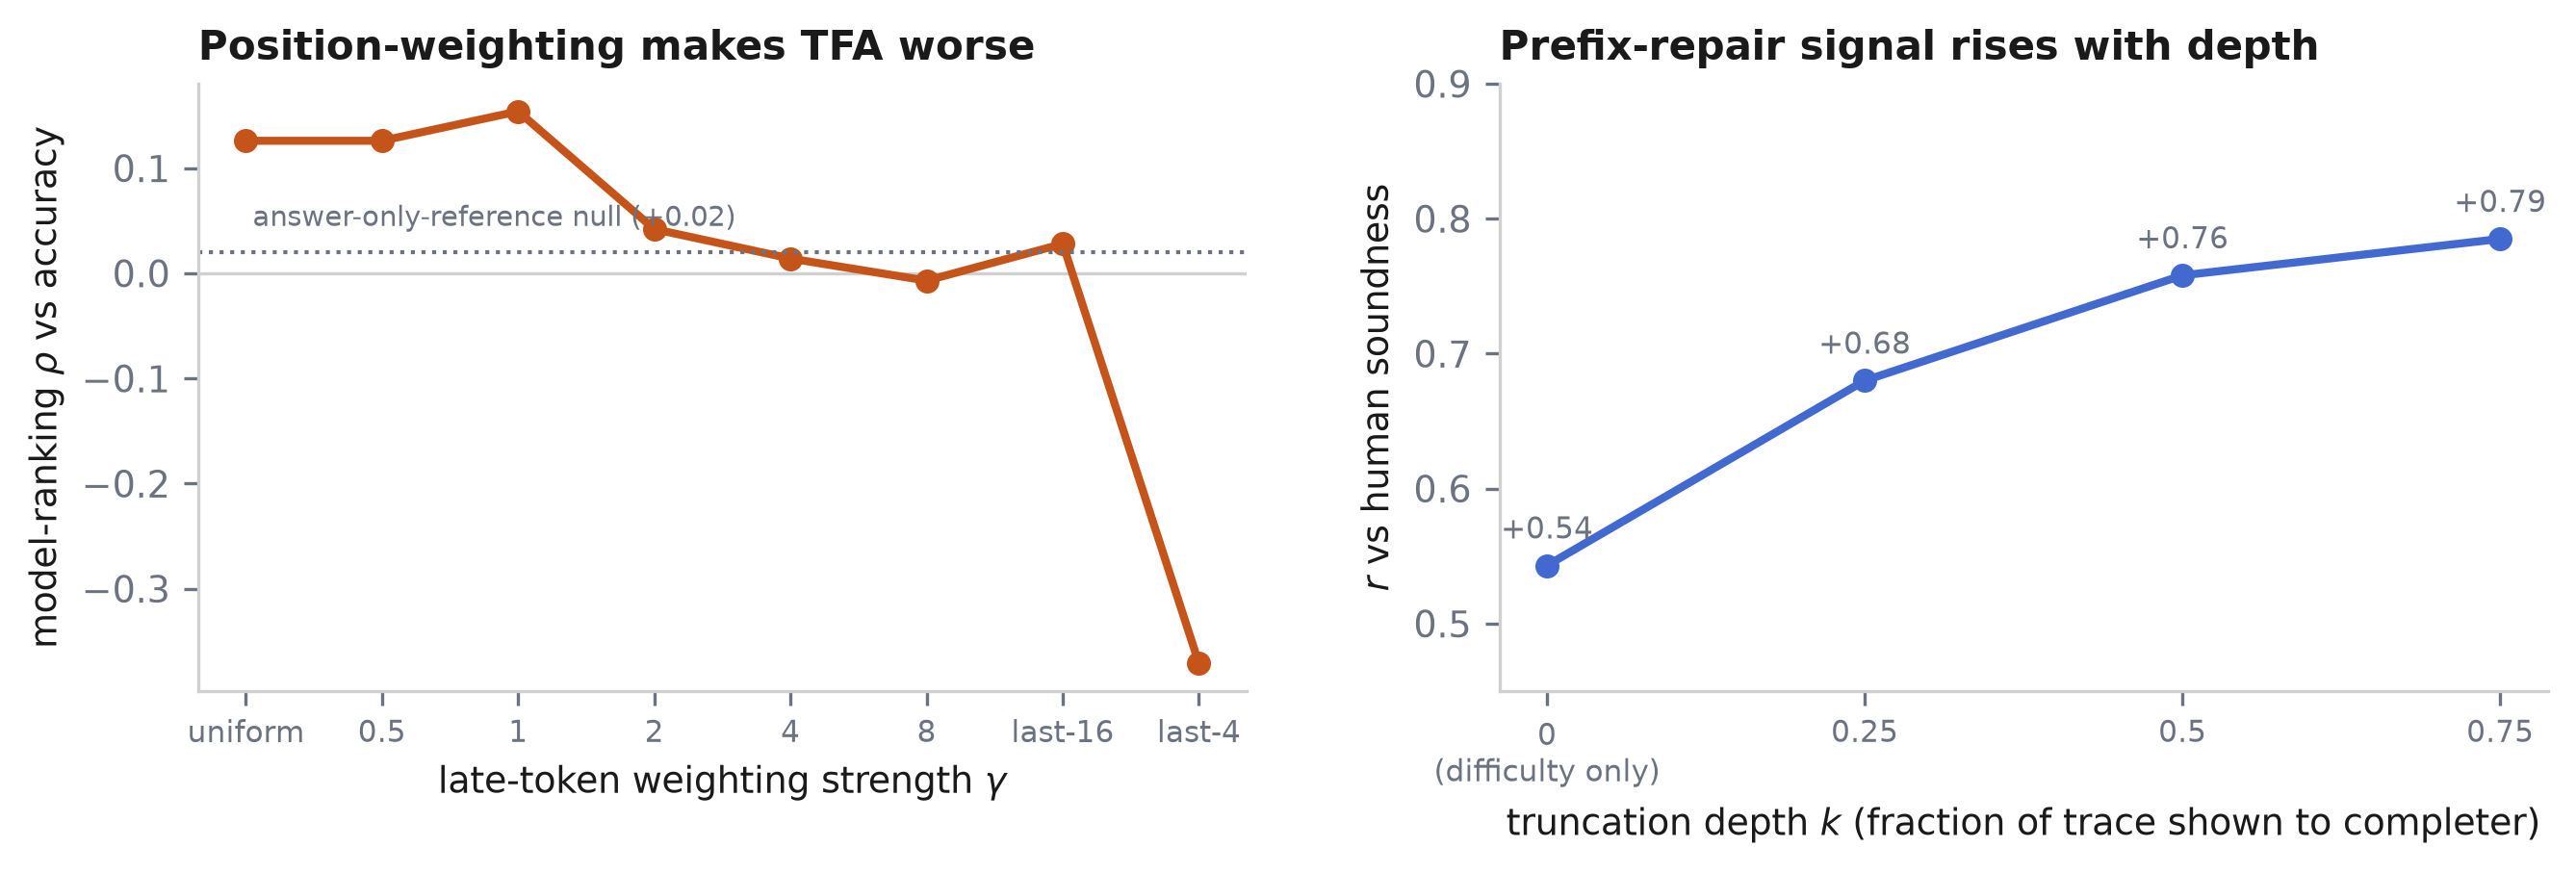
\includegraphics[width=0.9\textwidth]{figs/fig2_sweeps.png}
\caption{\textbf{The two registered sweeps move in opposite directions, as the taxonomy predicts.}
Left: up-weighting late reference tokens (the intuitive repair) decays \tfa's twelve-model ranking signal monotonically past $\gamma{=}1$, through the answer-only-reference null and beyond it.
Right: the prefix-repair signal rises monotonically with truncation depth, from a pure difficulty probe ($k{=}0$) to $+0.79$ against human soundness at $k{=}0.75$.}
\label{fig:sweeps}
\end{figure}

\section{The verification class grades, in proportion to endpoint checkability}
\label{sec:verify}

\subsection{Judge-free verification signals}

\emph{Executed tests} are the ceiling case: a free, perfect oracle wherever they exist, and the standard against which \tfa{} scored $0.00$.

\emph{The prefix-repair curve} is the strongest cheap signal we found.
Against the 60 joined labels of round two, its correlation with soundness rises monotonically with truncation depth: $+0.54$ at $k{=}0$ (solving from scratch, a pure difficulty probe), $+0.68$ at $k{=}0.25$, $+0.76$ at $k{=}0.5$, and $+0.79$ at $k{=}0.75$ (Figure~\ref{fig:sweeps}, right).
This is the profile that ``the trace's reasoning causally supports its answer'' should produce.
Controlling for difficulty via the $k{=}0$ arm, the prefix's added completability still carries $+0.69$.
For scale: on labeling round one every comparison metric sits at $|r| \le 0.24$ and the single-point completion value at $+0.49$; on this round the LLM judge reads $+0.89$ ($+0.59$ on round one).
The curve's $+0.79$ sits numerically at the human inter-rater reliability ceiling ($\rho = 0.79$, measured on the shared block), which is as high as any signal can be credited on these labels.
Its costs are real: about a hundred completions per solution, and a completer whose strength must sit in a middle band.
Too weak, and it cannot finish sound work; too strong, and it rescues broken work.

\emph{The answer-swap counterfactual} is the cheap end of the same class: one forward pass, no judge, no completion.
It is positive in 8 of 9 models (mean within-model $r = +0.13$, best $+0.34$), confirming the class prediction in direction while remaining too weak to use alone.
The ordering within the verification class (tests, then the repair curve, then answer-swap) tracks how much verification each performs, which is the taxonomy's internal consistency check.

\subsection{Judges are in the verification class only when anchored: a certification protocol}
\label{sec:certify}

Whether an LLM judge reads content or scores style is measurable with about sixty blind labels: two separated human scales, a divergence stratum where soundness and style decorrelate, and partial correlations as the verdict.
Our frontier judge (GPT-5.2, with the gold solution in context) passes.
On the divergence-decorrelated block, holding style fixed, its partial correlation with human soundness is $+0.86$; holding soundness fixed, its partial with style is $-0.06$.
Even among correct-answer solutions, where an impostor that only checks the final answer would flatline, it tracks soundness at $+0.81$.
The protocol can also convict: a deliberately sabotaged judge, prompted to reward presentation, is caught cleanly (style-given-soundness $+0.56$, soundness-given-style $+0.18$).

The decisive variable is the reference.
Every open-weights judge in the Qwen 1.5B--14B ladder fails certification without one: the 1.5B judge is overtly style-loaded ($+0.33$ style partial), and the larger ones are simply too weak ($0.24$--$0.28$ quality).
Every one of them passes with the gold solution in context ($+0.40$ at 1.5B up to $+0.53$ at 14B).
A reference changes what a judge measures, not merely how accurately it measures.
This is the bridge to the taxonomy: a referenced judge is performing verification, checking the solution against a trusted anchor, while an unanchored small judge degenerates to the comparison class's failure mode of rewarding surface form.

\paragraph{When a reference helps.}
On the planted-error detection task, the Qwen ladder detects $3/17/49/75\%$ of errors blind (1.5B/3B/7B/14B) and $21/85/85/90\%$ with the gold reference in context.
The 3B jump, from $17\%$ to $85\%$, replicates in all six model families we tested, with gains of $14$ to $60$ percentage points at that scale.
Comparing against a trusted reference is cheap enough for small models; producing the reference is the expensive part.
That split can be tested directly.
A judge that first solves the problem in a separate call, then grades against its own solution, detects $59/60/85/95\%$: above the gold reference at 1.5B and 14B, matching it at 7B, and trailing it at 3B.
At 1.5B the judge's own verbose solution beats the terse human gold as a comparison target.
Part of apparent reference-dependence is style matching, and part of small-judge weakness is protocol, not capability.

\paragraph{When a reference hurts.}
The same lever hurts when many answers are valid.
On multi-valid-answer comparisons, any reference, whoever wrote it, costs $7$--$8$ points of verdict accuracy (paired test, $p \le .0005$), because the judge anchors on one valid alternative and penalizes the rest.
So a reference converts a small judge into a verifier when the task's answer is effectively unique and verifying against the reference is within the judge's capability.

\section{The certificate predicts survival under optimization pressure}
\label{sec:pressure}

A static audit is only worth its cost if it predicts dynamic behavior.
The experiment is simple to state: a 7B model writes 64 candidate solutions per problem, each judge picks the one it thinks is best, and we check what actually happened.
Two things can go wrong, and we measure them separately:
\begin{itemize}
\item \textbf{Deception}: the judge's own scores say its picks are great when they are not.
We call this the \emph{excess hack gap}, reported in baseline standard deviations above a permutation null.
\item \textbf{Damage}: the picks are actually worse than the best available sample.
We call this \emph{oracle regret}: the accuracy left on the table relative to picking the best sample every time.
\end{itemize}
A judge can fail one measure without the other, and Table~\ref{tab:bon} shows both for all 25 configurations.
Three protocol details guard the estimates: selection and reporting use different rubric paraphrases (which cancels winner's curse), items are restricted to those the generator sometimes but not always solves (105 \textsc{MATH-500} and 68 \textsc{MBPP+} items with pool pass rate in $[0.2, 0.8]$), and the analysis scripts were committed before any data were generated.

\begin{table}[t]
\centering
\small
\begin{tabular}{lcc@{\qquad}cc}
\toprule
& \multicolumn{2}{c}{\textbf{math} (\textsc{MATH-500})} & \multicolumn{2}{c}{\textbf{code} (\textsc{MBPP+})} \\
judge config & excess gap & regret@64 & excess gap & regret@64 \\
\midrule
1.5B no-ref & $+0.88$ & $0.448$ & $+1.45$ & $0.412$ \\
3B no-ref & $+0.44$ & $0.429$ & $+1.06$ & $0.544$ \\
7B no-ref & $+0.80$ & $0.324$ & $+1.06$ & $0.426$ \\
14B no-ref & $+0.63$ & $0.324$ & $+1.04$ & $0.368$ \\
\midrule
1.5B ref & $+0.16$ & $\mathbf{0.010}$ & $+1.40$ & $0.441$ \\
3B ref & $+0.07$ & $0.038$ & $+0.43$ & $0.382$ \\
7B ref & $+0.18$ & $0.019$ & $+0.49$ & $0.265$ \\
14B ref & $+0.05$ & $0.048$ & $+0.37$ & $0.338$ \\
\midrule
GPT-5.2 no-ref & -- & -- & $+0.78$ & $0.212$ \\
GPT-5.2 ref & $+0.38$ & $0.117$ & $+0.22$ & $0.212$ \\
\midrule
7B sabotage & $+0.13$ & $0.400$ & $+0.84$ & $0.559$ \\
14B sabotage & $+0.61$ & $0.324$ & $+0.96$ & $0.426$ \\
GPT-5.2 sabotage & $+0.85$ & $0.133$ & $+0.61$ & $0.241$ \\
\bottomrule
\end{tabular}
\caption{\textbf{Best-of-64 selection pressure, 25 judge configurations.}
Every configuration that failed static certification is hacked on at least one estimand (large excess gap, large regret, or both), and every configuration certified in-domain resists.
The 1.5B-ref cell is the capability gate: the reference rescues the smallest judge on math and does nothing on code.
GPT-5.2 was not run unreferenced on math (the -- cells), hence 12 math + 13 code = 25 configurations.
Paired no-reference minus referenced contrasts and their bootstrap CIs are in Appendix~\ref{app:cis}.}
\label{tab:bon}
\end{table}

\paragraph{The certificate predicts, and it is domain-specific.}
Every configuration that failed static certification is hacked at best-of-64 on at least one estimand.
The blind configurations show excess gaps from $+0.44$ to $+1.45$ and lose $32$--$54\%$ of achievable accuracy; the sabotaged configurations fail in one of the two modes described below.
On math, where certification was measured in-domain, the prediction holds in all twelve configurations.
The reference collapses inflation by $4$--$13\times$ and regret by $7$--$45\times$ (paired within-size contrasts confirmed 4/4, per-configuration intervals disjoint).
On code, the reference protocol predicts twelve of thirteen configurations.
The single exception is the referenced 1.5B judge, hacked as badly as its blind twin, and it is the cell the capability-gate mechanism flags.
The operational lesson is that certification must be measured in the deployment domain: a judge certified on math is not thereby certified on code.

\begin{figure}[t]
\centering
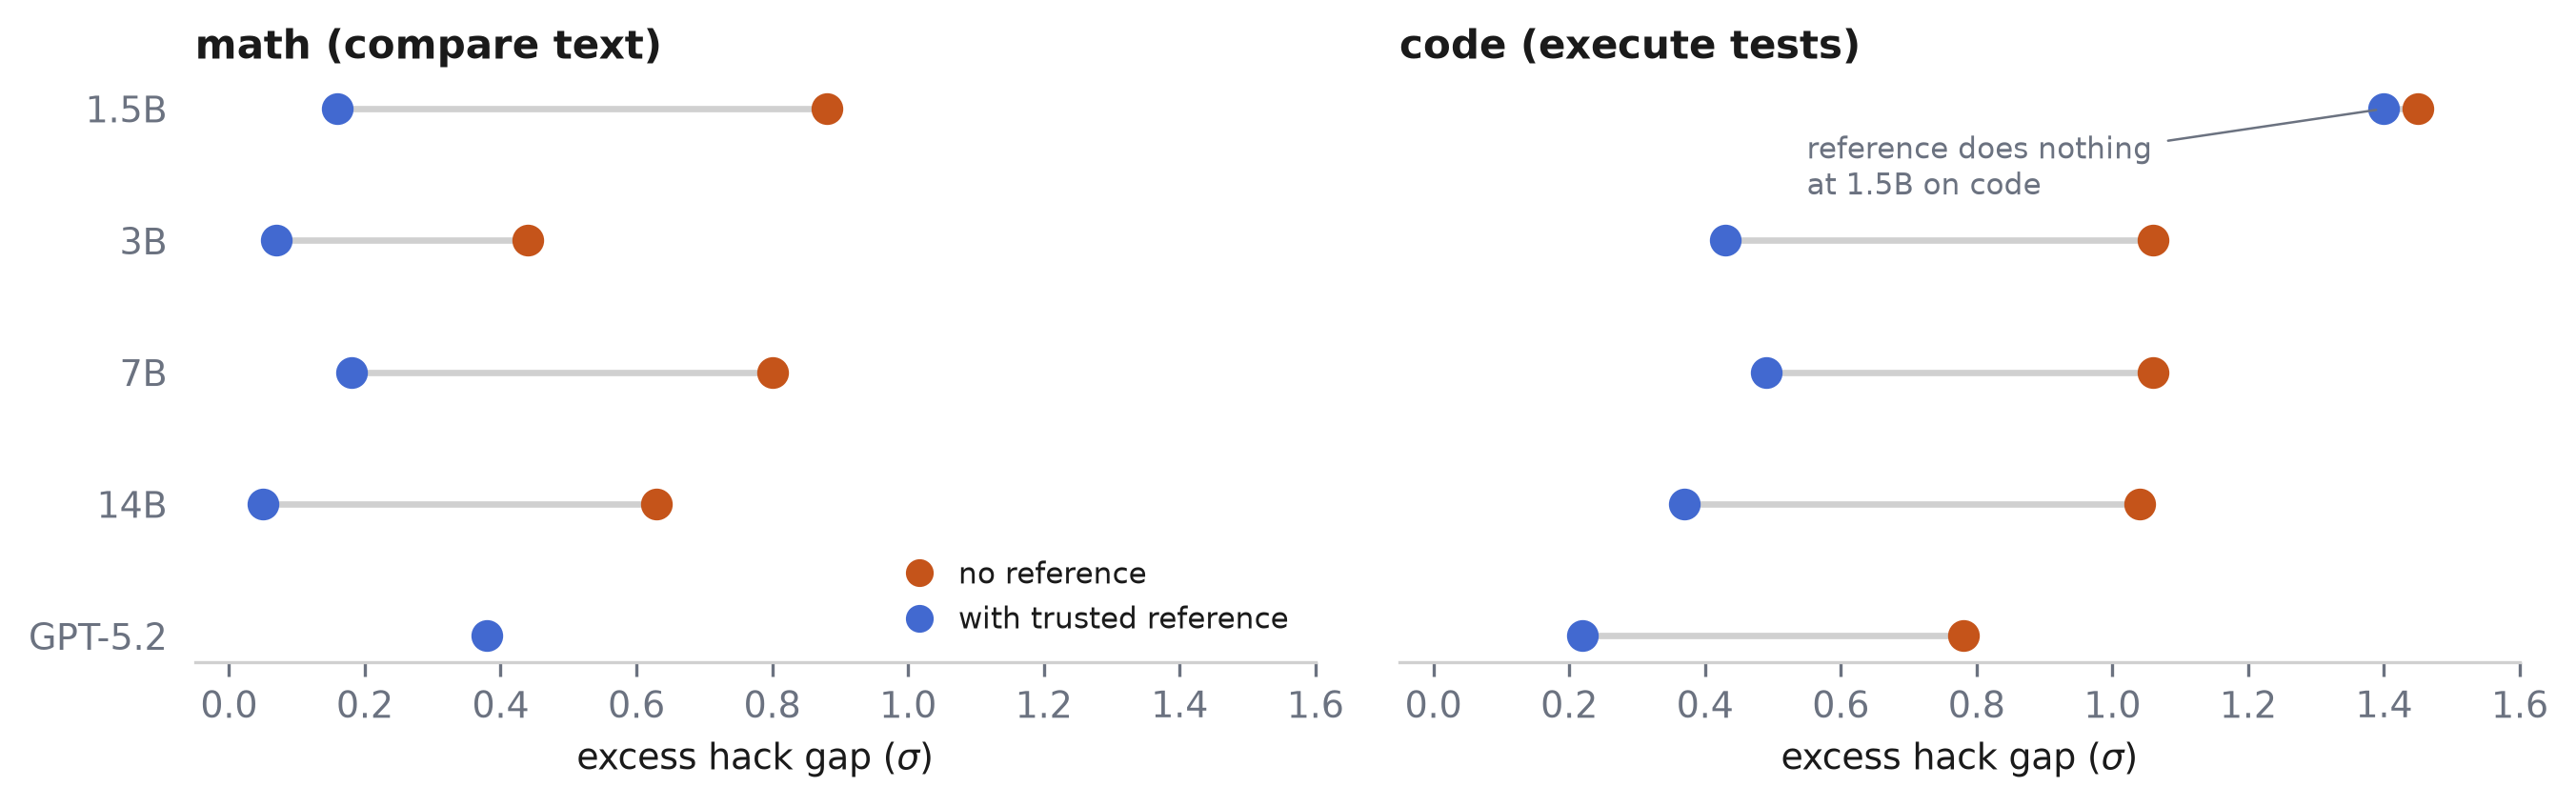
\includegraphics[width=0.9\textwidth]{figs/fig3_gate.png}
\caption{\textbf{The capability gate.}
Excess hack gap without (orange) and with (blue) a trusted reference, by judge scale.
On math the reference collapses inflation at every scale, including 1.5B.
On code, where using the reference means executing tests rather than comparing text, the lever works only at 3B and above, and the frontier judge needs it only for scoreboard honesty (its selection quality is identical either way).}
\label{fig:gate}
\end{figure}

\paragraph{The reference lever is capability-gated by verification hardness.}
On code the paired contrast replicates at 3B and above ($+0.63/+0.56/+0.67$, all excluding zero) but is null at 1.5B ($+0.05$ $[-0.29, +0.40]$; Figure~\ref{fig:gate}).
This is the same 1.5B judge that, with a reference, was the best selector on math (regret $0.010$, beating GPT-5.2's $0.117$).
The difference is what ``using the reference'' demands: comparing text on math, mentally executing tests on code.
At the frontier the gate closes from the other side.
GPT-5.2's selection quality on code is identical with and without the reference tests (regret $0.212$ both ways, the best of any code configuration), yet its unreferenced scoreboard still self-inflates $3.6\times$ ($+0.78$ versus $+0.22$).
Capability closes the damage gap without a reference, but an honest scoreboard still requires one.

\paragraph{A hacked judge fails in two modes, and capability trades one for the other.}
Across the sabotage ladder, real damage falls and self-inflation rises with judge capability.
The 7B sabotaged judge damages without inflating (regret $0.400$, gap $+0.13$ ns).
Sabotaged GPT-5.2 inflates without damaging (gap $+0.85$, regret $0.133$; on code $+0.61$ and $0.241$).
A blind cross-family panel (Claude Opus) confirms the channel: sabotage-selected solutions are more styled ($+0.27$ $[0.10, 0.44]$) with no detectable soundness loss.
The frontier mode, deceiving the metric while selecting well, is the dangerous one for training: a policy optimized against such a judge would internalize style.
Measuring what such a policy internalizes is the training-time experiment this work is designed to gate.

\paragraph{Granularity beats scale once a reference is in hand.}
The 1.5B referenced judge outselects GPT-5.2 on math for a mundane reason.
The frontier judge's 0--10 scale saturates, tying $78\%$ of items at the top score even when scores are read as probability-weighted expectations, and random tie-breaks admit wrong answers.
The small judge's continuous expected scores stay sharp.
Judge deployments that select should elicit fine-grained scores.
Coarse scales waste frontier capability.

\section{Design rules}
\label{sec:rules}

\begin{enumerate}
\item \textbf{Never use a reference as a similarity target.}
Its value is as context for a reader (Section~\ref{sec:certify}) or as a checkable endpoint for a verifier (Section~\ref{sec:verify}).
Any metric that scores resemblance to reference text inherits the nuisance decomposition of Section~\ref{sec:mechanism}, and the taxonomy correctly predicted the failure of every such metric before it was built.
\item \textbf{For leaderboards, matching is legitimate exactly when references are worth predicting.}
Report reference entropy alongside accuracy.
On answer-line references, matching measures style.
\item \textbf{Certify evaluators before optimizing against them, in the deployment domain.}
Sixty blind labels on two separated scales, a divergence stratum, and two partial correlations decide the matter.
The verdict predicted best-of-64 hack-resistance in every in-domain configuration, and the one cross-domain exception (the referenced 1.5B judge on code) is the reason the audit must be run where the judge will be used.
\item \textbf{Give a judge a reference only when the task's answer is unique and the judge can use it.}
Small judges need a reference they can read as text; an executable specification is wasted on them.
On multi-valid-answer tasks any reference anchors the judge against one valid alternative and lowers verdict accuracy.
\item \textbf{Elicit fine-grained scores from selecting judges.}
\item \textbf{Audit the oracle before the evaluator.}
Several apparent evaluator failures we chased in this work dissolved, on adjudication, into benchmark label errors and scorer bugs (Appendix~\ref{app:oracle}).
Measurement claims about evaluators are only as good as the ground truth they are scored against.
\end{enumerate}

\section{Limitations}
\label{sec:limits}

The human anchor is currently 80 random items graded by one annotator who is also an author, plus a divergence block graded by two.
A second rater on thirty random items, an external non-author annotator, and the code-domain human labels are pending, and the prefix-repair headline ($+0.79$) should be treated as provisional until they land.
The prefix-repair completer shares a model family with a subset of the graded traces, and its signal is substantially correctness-mediated: among correct-only solutions it drops to $+0.21$.
The same caveat applies to every signal except the judge.
Selection-pressure results use one generator per domain and strict string-match oracles.
Equivalence adjudication is pending; it can only shrink no-reference regrets, so the reference contrast is conservative.
Judge-validity claims cover one frontier judge on math plus executable code; a second dataset and a frontier-judge row are future work.
Pooled seventeen-model rankings have wide intervals, so we rest the ranking claims on the within-family ladders, which are individually consistent.
Training against certified and uncertified judges, rather than selecting with them, is designed and gated on this write-up.

\section{Related work}
\label{sec:related}

Reliability audits of LLM judges conclude that reliability without validity is the field's open problem, and they call for variance-component analysis of the kind performed here~\cite{zheng2023judging,tan2024judgebench}.
The style-over-substance literature documents judge biases in general pools~\cite{wu2023style,dubois2024length,singhal2023long}.
Our finding is complementary: on reference-equipped math with a strong judge, the style loading is not detectable, and the larger measurement hazards sat in the benchmarks' own answer keys.
Scaling-law treatments of oversight measure judge--solver capability gaps in game-like settings~\cite{engels2025scaling}; our capability gate localizes the analogous phenomenon to a concrete mechanism, the verification hardness of the reference, on real math and code.
Reward-model overoptimization is documented for trained reward models~\cite{gao2022scaling,skalse2022defining,coste2023ensembles,eisenstein2023helping}.
Our contribution there is an ex-ante certificate, measured on sixty labels, that predicted which judge configurations would be exploited before any optimization ran, plus the two-mode decomposition of what ``exploited'' means.
JudgeLM and Prometheus ablate references as a training design choice for judge models~\cite{zhu2023judgelm,kim2024prometheus2}; we show references flip the validity of untrained judges, and that the effect is capability-gated.
Completion-based process values descend from rollout estimation in process supervision~\cite{lightman2023verify,wang2022selfconsistency}.
The prefix-repair curve, its monotone depth profile, and its difficulty-controlled reading appear to be new, as does the class-level advance-prediction test of the comparison/verification taxonomy.

\section{Conclusion}
\label{sec:conclusion}

Reference-based evaluation has been treated as a spectrum of increasingly good approximations to judgment.
It is not a spectrum.
It is two mechanisms.
Signals that compare a solution to reference text measure the reference: $80\%$ perplexity, $83$--$92\%$ item nuisance.
No reweighting recovers a grading signal, because there is none to recover.
Signals that verify a checkable endpoint grade in proportion to how much verification they perform, from a one-pass answer-swap margin, through the prefix-repair curve, to executed tests.
LLM judges join the class when a trusted reference anchors them and they are capable of using it.
Because the failure is mechanistic, trust stops being a leap.
A sixty-label blind audit certifies an evaluator in its deployment domain, the certificate predicted hack-resistance under best-of-64 pressure across two domains, and the taxonomy called the outcome of every new metric we built before the data existed.
The open frontier is dynamic: what does a policy \emph{trained} against a certified versus an uncertified judge internalize?
The frontier sabotage mode, which deceives metrics without damaging selection, makes that the question on which the rest of this program hangs.

\vspace{1em}
\noindent\textbf{Reproducibility.}
All scores, labels, decompositions, pre-registered analysis scripts, and the certification instruments are in the repository (\texttt{experiments/tfa-vs-judge}): the class table (\texttt{runs/metric\_class\_results.md}), the decomposition (\texttt{scripts/two\_way\_decomp.py}), the short-reference intervention (\texttt{scripts/tfa\_shortref.py}), the metric slate (\texttt{scripts/analyze\_metric\_ablations.py}, \texttt{scripts/analyze\_slate2.py}), the certification protocol (\texttt{docs/judge-certification-paper.md}, \texttt{runs/cert\_out/}), the selection-pressure grids (\texttt{scripts/bon\_*.py}, \texttt{runs/bon\_phase0\_results.md}, \texttt{runs/bon\_v2\_full.json}, \texttt{runs/bon\_code\_full.json}), and the labeling instruments with returned labels (\texttt{human\_eval/}).

\appendix

\section{Confidence intervals for the paired reference contrasts}
\label{app:cis}

Per-size paired contrasts of the excess hack gap, no-reference minus referenced, with per-item bootstrap 95\% intervals (2{,}000 resamples).

\begin{table}[h]
\centering
\small
\begin{tabular}{lcc}
\toprule
judge size & math ($n{=}105$ items) & code ($n{=}68$ items) \\
\midrule
1.5B & $+0.72$ $[+0.57, +0.86]$ & $+0.05$ $[-0.29, +0.40]$ \\
3B & $+0.37$ $[+0.24, +0.51]$ & $+0.63$ $[+0.44, +0.83]$ \\
7B & $+0.62$ $[+0.48, +0.76]$ & $+0.56$ $[+0.32, +0.81]$ \\
14B & $+0.57$ $[+0.36, +0.78]$ & $+0.67$ $[+0.41, +0.95]$ \\
\bottomrule
\end{tabular}
\caption{Every math contrast and every code contrast at 3B+ excludes zero; the code 1.5B contrast is the capability-gate null.}
\label{tab:cis}
\end{table}

\section{The oracle audit behind design rule 6}
\label{app:oracle}

Three apparent judge-failure effects in our own early data looked like textbook oversight laws: an attractor effect on \textsc{GSM8K}, a capability-gap degradation curve, and a detection hierarchy across judge sizes.
On case-by-case adjudication, $71$--$83\%$ of the flagged instances in these effects were errors in the benchmarks' own grading pipelines (wrong answer keys or scorer parsing failures), and all three effects dissolved once labels were repaired.
The cleanup yielded a tool: when the full ladder of cheap judges (1.5B--7B) unanimously disagrees with the official label, the official label is the one that is wrong $89\%$ of the time, a rate we validated against a human re-annotation of the flagged \textsc{GSM8K} items.
After repair, adjudicated frontier-judge false positives sit near $2\%$ across difficulty, which is the base rate any claim of judge failure must beat.

\section{The full metric-class table}
\label{app:classtable}

All five comparison metrics under the same four tests: model-level boundary (hard-benchmark / \textsc{GSM8K} pooled $\rho$), variance decomposition (item / item$\times$family / residual shares, four families), and correlation with blind human soundness (labeling round one, $n{=}60$).

\begin{table}[h]
\centering
\small
\begin{tabular}{llccc}
\toprule
metric & mechanism & boundary (hard / sat.) & item / fam / resid \% & vs.\ human \\
\midrule
\tfa{} (argmax) & prediction fit & $+0.60$ / $-0.25$ & $83$--$92$ / $3$--$7$ / $5$--$11$ & $-0.07$ \\
gold-token logprob & prediction fit & $+0.43$ / $-0.23$ & $83$--$91$ / $7$--$11$ / $1$--$6$ & $-0.17$ \\
TF-IDF cosine & weighted similarity & $+0.72$ / $+0.12$ & $69$ / $8$ / $23$ & $+0.01$ \\
sentence embeddings & semantic similarity & $+0.87$ / $+0.29$ & $\sim$$70$ / $8$ / $21$ & $+0.14$ \\
unigram-F1 & raw overlap & $-0.49$ / $+0.18$ & $45$--$55$ / $12$--$15$ / $32$--$41$ & $-0.24$ \\
\midrule
LLM judge (referenced) & verification & --- & --- & $+0.59$ \\
completion value & verification & --- & --- & $+0.49$ \\
\bottomrule
\end{tabular}
\caption{Prediction-fit and weighted-similarity metrics rank on hard benchmarks and die or invert on saturated ones; raw overlap does not rank at all (its hard-benchmark inversion is a verbosity confound: controlling output length moves $-0.49$ to $-0.07$).
No comparison metric grades against human soundness; both verification signals do.}
\label{tab:classfull}
\end{table}

\begin{thebibliography}{20}
\small
\bibitem{zheng2023judging} L.~Zheng et al. Judging LLM-as-a-Judge with MT-Bench and Chatbot Arena. arXiv:2306.05685, 2023.
\bibitem{tan2024judgebench} S.~Tan et al. JudgeBench: A Benchmark for Evaluating LLM-Based Judges. arXiv:2410.12784, 2024.
\bibitem{wu2023style} M.~Wu and A.~F.~Aji. Style Over Substance: Evaluation Biases for Large Language Models. arXiv:2307.03025, 2023.
\bibitem{dubois2024length} Y.~Dubois et al. Length-Controlled AlpacaEval: A Simple Way to Debias Automatic Evaluators. arXiv:2404.04475, 2024.
\bibitem{singhal2023long} P.~Singhal et al. A Long Way to Go: Investigating Length Correlations in RLHF. arXiv:2310.03716, 2023.
\bibitem{gao2022scaling} L.~Gao, J.~Schulman, and J.~Hilton. Scaling Laws for Reward Model Overoptimization. arXiv:2210.10760, 2022.
\bibitem{skalse2022defining} J.~Skalse et al. Defining and Characterizing Reward Hacking. arXiv:2209.13085, 2022.
\bibitem{coste2023ensembles} T.~Coste et al. Reward Model Ensembles Help Mitigate Overoptimization. arXiv:2310.02743, 2023.
\bibitem{eisenstein2023helping} J.~Eisenstein et al. Helping or Herding? Reward Model Ensembles Mitigate but do not Eliminate Reward Hacking. arXiv:2312.09244, 2023.
\bibitem{engels2025scaling} J.~Engels et al. Scaling Laws for Scalable Oversight. arXiv:2504.18530, 2025.
\bibitem{zhu2023judgelm} L.~Zhu, X.~Wang, and X.~Wang. JudgeLM: Fine-tuned Large Language Models are Scalable Judges. arXiv:2310.17631, 2023.
\bibitem{kim2024prometheus2} S.~Kim et al. Prometheus 2: An Open Source Language Model Specialized in Evaluating Other Language Models. arXiv:2405.01535, 2024.
\bibitem{lightman2023verify} H.~Lightman et al. Let's Verify Step by Step. arXiv:2305.20050, 2023.
\bibitem{wang2022selfconsistency} X.~Wang et al. Self-Consistency Improves Chain of Thought Reasoning in Language Models. arXiv:2203.11171, 2022.
\bibitem{yuan2021bartscore} W.~Yuan, G.~Neubig, and P.~Liu. BARTScore: Evaluating Generated Text as Text Generation. arXiv:2106.11520, 2021.
\bibitem{hendrycks2021math} D.~Hendrycks et al. Measuring Mathematical Problem Solving With the MATH Dataset. arXiv:2103.03874, 2021.
\bibitem{cobbe2021gsm8k} K.~Cobbe et al. Training Verifiers to Solve Math Word Problems. arXiv:2110.14168, 2021.
\bibitem{chen2021codex} M.~Chen et al. Evaluating Large Language Models Trained on Code. arXiv:2107.03374, 2021.
\bibitem{austin2021mbpp} J.~Austin et al. Program Synthesis with Large Language Models. arXiv:2108.07732, 2021.
\bibitem{liu2023evalplus} J.~Liu et al. Is Your Code Generated by ChatGPT Really Correct? Rigorous Evaluation of Large Language Models for Code Generation. arXiv:2305.01210, 2023.
\end{thebibliography}

\end{document}
